% REVISION PROPOSAL (DEC-065). NOT the definitive manuscript.
% Original manuscript: Paper_manuscript/main.tex, git blob afbaf86...: `git rev-parse 0db386b:Paper_manuscript/main.tex` = afbaf8616444d8d416d051fe5f566af6527e8f3575 (unchanged).
% Every number below comes from a stored artifact (IEEE39_DEC062_*, DEC063_*, DEC064_*, DEC065_*). Items marked \todo{} need the investigator's review.
\documentclass[11pt,twocolumn]{article}

\usepackage[utf8]{inputenc}
\usepackage{amsmath}
\usepackage{amssymb}
\usepackage{bm}
\usepackage{graphicx}
\usepackage{booktabs,array}
\usepackage{hyperref}
\usepackage[margin=0.9in]{geometry}

\newtheorem{theorem}{Theorem}
\newtheorem{proposition}{Proposition}
\newtheorem{lemma}{Lemma}
\newtheorem{corollary}{Corollary}
\newtheorem{remark}{Remark}
\newtheorem{assumption}{Assumption}
\newenvironment{proof}{\par\noindent\textit{Proof.}\ }{\hfill$\square$\par}
\newcommand{\todo}[1]{\textbf{[REVIEW: #1]}}
\newcommand{\UD}{U_{\mathrm{D8}}}

\title{Post-Disturbance Capability Admissibility and Preventive Dispatch for Distributed Frequency--Voltage Control}
\author{AUTHORS}

\begin{document}
\sloppy
\maketitle

\begin{abstract}
Distributed secondary controllers can keep the references of generating units inside their capability sets, but the power that each unit actually delivers at the instant of a disturbance is fixed by the pre-event dispatch. For a differential--algebraic plant, we show that, under continuity of states and control actions at the event, the post-event unit margins are independent of the controller (Theorem~\ref{thm:ta}), which yields a necessary admissibility condition, and we bound the influence of a rate-limited controller on the following $50$~ms for the linearised plant (Proposition~\ref{prop:os}); a nonlinear bound is not obtained. We design a preventive dispatch with a sub-cycle margin predictor and evaluate it on a modified IEEE 39-bus system with synchronous and grid-forming units, using a protocol with frozen code and registered predictions. The evaluation of the final design was run under an access rule modified after tuning, and the original gate is not met. In the 9 blind cells of the operating condition with redispatch, 7 are safe and 2, at bus 31, are inadmissible at the jump (the S2 cell fails for all four controllers compared); without redispatch, 2 cells predicted safe are unsafe after $50$~ms. We also study a centered distributed controller driven by a supervisory equilibrium target, for which discrete-time reference invariance and conditional local stability are proved; a barrier/Lyapunov quadratic program added to it shows no measurable effect beyond rate limiting. The claims are limited to the tested network, step disturbances and the stated information assumptions.
\end{abstract}

\section{Introduction}
\label{sec:intro}
Distributed secondary frequency and voltage controllers for networks with synchronous generators (SGs) and inverter-interfaced resources are commonly required to respect unit capability limits. Existing designs enforce these limits on the controller references: the resilient distributed controller (RDC) of Kavvathas and Konstantopoulos keeps the active/reactive set-points inside each capability set by an invariance argument \cite{Kavvathas2025Resilient,Kavvathas2023MED}; projected primal--dual designs keep power references inside capacity sets during transients \cite{Wang2026Distributed,Mo2026MultiSlot}; barrier-function correctors have been added to secondary frequency control \cite{MoLiu2025Transient,Tang2026SafeFrequency}. Frequency-secured scheduling constrains the nadir and the rate of change of frequency at system level \cite{Paturet2020Stochastic}, and a recent survey frames preventive scheduling and the post-contingency initial condition as a joint object \cite{She2026Security}.

\emph{Gap.} In the works we examined (Sec.~\ref{sec:lit}), the constraint enforced by the controller is a constraint on its references. The power delivered by a unit at the instant of a step disturbance is an algebraic variable of the network and jumps at the event; its margin is set by the pre-event dispatch, whatever the secondary controller does afterwards. We did not find, among the works examined, a treatment of this instant as a condition on the dispatch for unit-level $P$, $Q$, $S$ and $V$ limits. The search was not exhaustive and we claim no priority.

\emph{Contributions}, in the order of their evidential strength:
\begin{enumerate}
\item A theorem (T-A) stating that, under explicit continuity hypotheses, the unit margins at the post-event instant do not depend on the controller, and the necessary admissibility condition that follows (N2). Proved.
\item A bound on the controller's influence over the first $50$~ms (Proposition~\ref{prop:os}) for the linearised differential--algebraic plant, with controller-specific rate bounds and a numerical validation; a nonlinear bound is not obtained.
\item A preventive dispatch with an overshoot-aware predictor (M3+OS), evaluated blind with its failures reported (Sec.~\ref{sec:results}).
\item A centered RDC with a supervisory equilibrium target: exact restoration at the selected equilibrium (Lemma~\ref{lem:c}), discrete-time reference invariance as an adaptation of known barrier conditions (Theorem~\ref{thm:t1}), and conditional local stability (Theorem~\ref{thm:t2}).
\item A classification of cells into proved, numerically verified and observed levels (P3), and the documentation of negative results.
\end{enumerate}
Section~\ref{sec:limits} lists what is not claimed.

\section{System Model and Physical Constraints}
\label{sec:model}
\subsection{Plant}
The plant is a differential--algebraic system
\begin{equation}
\dot x=f(x,y,u,d),\qquad 0=g(x,y,u,d),
\label{eq:dae}
\end{equation}
with dynamic states $x$ (including SG rotor, excitation and governor states), algebraic variables $y$ (network voltages and unit powers), references $u=(P^s,Q^s)\in\mathbb R^{2n}$ of the $n=10$ units and the constant disturbance $d$. Quasi-algebraic states are absorbed in $y$. We assume (H-DAE) that $g_y$ is nonsingular on the region visited, so that $y=\psi(x,u,d)$ and $\dot x=F(x,u,d)$. The case is the IEEE 39-bus network with ten units in a hybrid SG--grid-forming configuration, simulated with ANDES 2.0.0 (trapezoidal rule, $\Delta t=2^{-8}$~s with local refinement $\Delta t/16$ on $[t_e-\Delta t,t_e+0.5]$~s, tolerance $10^{-4}$) \cite{Kavvathas2025Resilient}\todo{cite the case/ANDES source used in the repository}.

\subsection{Limits and margins}
For each unit $i$ the delivered quantities $P_i,Q_i,S_i=\sqrt{P_i^2+Q_i^2},V_i$ are subject to limits. Writing $h_j(x,y,u)\ge 0$ for the margin of constraint $j$ (limit minus value), a \emph{violation} is $h_j<0$; this is a modelling definition of delivered-quantity limits, not of turbine-side limits. The reference set is
\begin{equation}
\mathcal W=\{u:c_j(u)\ge0\},\quad c_5=s_i^2-(P_i^s)^2-(Q_i^s)^2,
\label{eq:W}
\end{equation}
with affine rows $c_1,\dots,c_4$ (active and reactive boxes) and, for SG units, $c_6,c_7$ (exciter clamp).

\subsection{Events and operating conditions}
The event is a step of a constant-power load at a bus. Three operating conditions OC1, OC2, OC3 correspond to 100\%, 90\% and 110\% of the base load; three amplitude levels S1$<$S2$<$S3 are used. The numerical uncertainty of a margin is $\UD=0.0109$~pu, estimated in the numerical audit of the algebraic jump.

\subsection{Controllers and information}
\label{sec:controllers}
All controllers act on $u$ through $u_{k}^{+}=u_k+h\,v_k$, applied before integrating the sample. B2 is the RDC of \cite{Kavvathas2025Resilient} with the gains and normalisation of the original design. B1s is a conventional integral controller with separate saturation (a comparator constructed for this study). B4$'$ is the centered RDC $v_{\rm nom}=v_{\rm RDC}(\xi)-v_{\rm RDC}(\hat\xi^\star)$ filtered by a quadratic program with a rate box and barrier rows; B5$'$ is B4$'$ plus a soft Lyapunov row. The centered controllers use a \emph{supervisory target} $\hat\xi^\star$: it is the pre-event equilibrium until $t_e+\tau_{\rm info}$ and the post-event equilibrium afterwards, $\tau_{\rm info}=1$~s (assumption A-INFO). B2 and B1s have no such information; \textbf{every comparison below is under equal events, dispatch and solver, not under equal information.}

\section{Post-Event Admissibility}
\label{sec:ta}
\begin{assumption}[H-C, continuity]
At the event, $x(t_e^+)=x(t_e^-)$ and $u(t_e^+)=u(t_e^-)$.
\end{assumption}
In the sampled implementation the first update of $u$ occurs before the step that contains $t_e$, so H-C holds up to $\eta$ with $|\eta_k|\le h\bar v_{c,k}$ ($\bar v_c$ the rate bound of controller $c$).

\begin{theorem}[Post-event admissibility, T-A]
\label{thm:ta}
Under H-DAE and H-C, any two controllers produce the same post-event outputs $y(t_e^+)=\psi(x^-,u^-,d^+)$, hence the same margins $h_j(t_e^+)=a_j(z,d^+)$, a function of the pre-event dispatch $z$ and the disturbance only.
\end{theorem}
\begin{proof}
Both trajectories share $(x(t_e^+),u(t_e^+),d^+)$; $y(t_e^+)$ is the solution of $g=0$ near the pre-event algebraic point, unique by the implicit function theorem.
\end{proof}
\begin{corollary}[N2]
If $a_j(z,d^+)<0$ for some $j$, every controller satisfying H-C violates constraint $j$ at $t_e^+$.
\end{corollary}
\begin{remark}
With the sampled update, $|h_j^a-h_j^b|\le\sum_k|C_{u,jk}|h(\bar v_{a,k}+\bar v_{b,k})$ plus a second-order remainder, where $C_u=\partial y/\partial u$; in this plant $\|C_u\|\approx10^{-16}$. The corollary is a consequence of the theorem: its confirmation in the experiments (Sec.~\ref{sec:results}) is a consistency check.
\end{remark}

\begin{proposition}[Influence after the jump, linearised plant]
\label{prop:os}
Let $(A,B,C_x,C_u)$ be the reduced matrices of the linearisation of \eqref{eq:dae} at the pre-event point and let two controllers satisfy $|u_k^a(s)-u_k^b(s)|\le s\,w_k$\ for $s\in[0,T]$\ after $t_e^+$, with $w_k=w^a_k+w^b_k$ the sum of their rate bounds. Then, for the linearised plant,
\begin{multline}
|\Delta y_j(T)|\le\sum_k w_k\Big(|C_{u,jk}|\,T\\
{}+\int_0^T\big|[C_xe^{A(T-s)}B]_{jk}\big|\,s\,ds\Big).
\end{multline}
\end{proposition}
\begin{proof}
Variation of constants and $|\Delta u_k(s)|\le s\,w_k$.
\end{proof}
\emph{Rate bounds per controller.} B5$'$, B4$'$: $|v_k|\le\bar v_k=0.01\,s_k$~pu/s by the box row. B1s: $v_{P,i}=k_i(1-\omega_i)\to0$ ($\omega_i$ is a state) and $v_{Q,i}=K_{IQ}K_V(V_i(0)-V_i)$ with $V_i$ algebraic, so its initial value equals the jump of $V_i$ fixed by Theorem~\ref{thm:ta}. B2: the RDC rate depends on the algebraic outputs, so $v(t_e^+)$ is computable from Theorem~\ref{thm:ta}, but no bound over the interval was derived; the measured $50$~ms maximum (up to $6.27\,\bar v$) is used and is empirical.

\begin{remark}[What is and is not established]
(i) For the linearised plant the statement is proved. (ii) For the nonlinear plant the same bound requires Lipschitz constants; with the norm constants of the frozen linearisation ($L_x\approx2.9\times10^4$~s$^{-1}$) the Gronwall bound overflows, so \emph{a nonlinear quantitative bound is not obtained}. (iii) Numerically, in 6 cells and 18 controller pairs, the bound holds in all pairs (0.8--1.8\,mpu against $\UD=10.9$\,mpu), and the linear model reproduces the observed output differences at $t_e+50$~ms (for example $3.82\times10^{-4}$ vs. $3.84\times10^{-4}$~pu); the observed unit-output differences reach $5.0\times10^{-4}$~pu. These matrices are estimates of a frozen linearisation, not certificates.
\end{remark}

\section{Preventive Dispatch and Overshoot Predictor}
\label{sec:dispatch}
Let $a_j(z,d)$ be the post-event margin of Theorem~\ref{thm:ta}. The preventive dispatch (M3+OS, Algorithm~1 of the repository) selects $z$ subject to the network equations and to $a_j(z,d)\ge\varepsilon_{\rm OS}+\UD$ for the design events, where $\varepsilon_{\rm OS}=3.88\times10^{-4}$~pu is an overshoot term calibrated on the design and tuning events (the sub-cycle overshoot of the margin beyond $a_j$ that a dense post-jump predictor resolves), with a cost on the redispatch. Events are partitioned into DESIGN (buses 8, 23, 28, 25), TUNE (7, 20, 16, 24) and TEST (21, 31, 39). A cell is classified SAFE if all margins are $\ge\UD$ and UNSAFE if one is $\le-\UD$; otherwise NUMERICALLY\_INDETERMINATE; after 50~ms and for $Q,S,V$ the classification is binary. A cell is \emph{eligible} (confirmatory) if the event is admissible at the jump. The OC1 design used in the evaluation is the third revision (rev3), obtained after the tuning stage. \todo{Algorithm 1 statement to be written from dec054\_opf; the text above is a summary.}

\section{Centered Distributed Regulation and Conditional Guarantees}
\label{sec:centered}
\subsection{Post-event equilibrium and supervisory information}
The target $\xi^\star=(x^\star,u^\star)$ solves: (E1) plant equilibrium for $d^+$ with one rotor angle anchored; (E2) proportional active sharing $P_i^\star=(1+\alpha)P_i^n$ except for units pinned at an $\epsilon_{\rm sel}=0.01$-interior band edge; (E3) unit-bus voltages at their dispatch set-points except for reactive-limited units; and (E4) admissibility checked after solving. The supervisor needs the pre-event state and dispatch, the load change (bus and magnitude) and the plant model; in the experiments the model is the ANDES model of the plant itself, so \emph{there is no model mismatch}, which favours the centered controllers.

\begin{lemma}[Centering]
\label{lem:c}
If $\xi^\star$ satisfies (E1) and the target is exact ($\hat\xi^\star=\xi^\star(d^+)$ of the actual plant), then $v_{\rm nom}(\xi^\star)=0$, $v=0$ is the unique minimiser of the filter, and $\xi^\star$ is a fixed point of the sampled loop.
\end{lemma}
\begin{proof}
$v_{\rm nom}(\xi^\star)=v_{\rm RDC}(\xi^\star)-v_{\rm RDC}(\xi^\star)=0$; $v=0$ is feasible by Theorem~\ref{thm:t1} (feasibility), and the objective is strictly convex; (E1) gives $\varphi_h(x^\star,u^\star)=x^\star$.
\end{proof}
Exactness of the target is needed: with a stale or mismatched target the fixed point moves, and robustness to mismatch is not covered. Lemma~\ref{lem:c} gives the steady state ($\omega=1$, voltages at set-points, proportional sharing) but not convergence.

\subsection{Reference invariance (discrete adaptation)}
\begin{theorem}[Discrete reference invariance]
\label{thm:t1}
Let $u_0\in\mathcal W$, $\gamma_k=\alpha h_k\in(0,1]$, $u_{k+1}=u_k+h_kv_k$ and $c_j(u_k+h_kv_k)\ge(1-\gamma_k)c_j(u_k)$ for all $j$ (for $c_5$ through the second-order cone). Then $c_j(u_k)\ge\prod_i(1-\gamma_i)\,c_j(u_0)\ge0$; and $v=0$ is feasible whenever $u_k\in\mathcal W$.
\end{theorem}
This is the discrete-time barrier condition used in sampled-data barrier functions \cite{Breeden2021Sampled}; the invariance of the reference set is already a property of the RDC \cite{Kavvathas2025Resilient}. We present it as an auxiliary adaptation to the centered, rate-limited, sampled law, \emph{not} as an original invariance result. T1 concerns references only and implies nothing about delivered $P,Q,V$. \todo{Whether the centering offset preserves the inward-pointing property of the original RDC is open; if it does, Theorem~\ref{thm:t1} is redundant in continuous time.}

\subsection{Conditional local stability}
\begin{theorem}[Local stability of the centered sampled RDC]
\label{thm:t2}
Under (H1) the target is a verified equilibrium, (H2) smoothness with inactive limiters, (H3) $c_j(u^\star)>0$, (H4) the sampled map has a simple unit eigenvalue (common angle) and all others strictly inside the unit disc, (H5) the continuous closed loop has a simple zero eigenvalue and the rest in the open left half-plane, there is a neighbourhood $N$ of $\xi^\star$ in which the filter returns $v_{\rm nom}$ and the sampled loop converges exponentially, modulo the common angle.
\end{theorem}
Proof: the filter rows are strictly satisfied at $v_{\rm nom}$ near $\xi^\star$ by (H3), so the loop is the centered RDC, whose map is $C^1$ with fixed point $\xi^\star$; the discrete indirect Lyapunov method gives the claim. H1, H4, H5 are verified in floating point, not certified; $N$ is not quantified; and membership of the state at $t_e+\tau_{\rm info}$ in $N$ is not certified. The statement is a property of the centered RDC: \emph{the QP and the Lyapunov row are inactive on $N$.}

\section{Experimental Design and Traceability}
\label{sec:design}
The protocol was frozen before the blind evaluation (code, parameters, criteria, classification rules, hashes; tag \texttt{dec062-freeze}); predictions, hypotheses and falsifiers were committed before the first blind simulation; all 54 evaluation runs were written after the sealing commit and their stored files match their hashes (\texttt{IEEE39\_DEC063\_audit.json}; local git clock, not externally notarised). The total budget was 120 time-domain simulations (TDS); 112 were used.

\textbf{Gate history.} The original gate G3 and the revised gate G-v2 were \emph{not met}: G-v2 is REJECTED because criterion (iv) (unit-voltage error $\le10^{-3}$~pu at 200~s) fails in three OC1 rev3 S3 cells (b7: $1.278\times10^{-3}$, b16: $1.015\times10^{-3}$, b24: $1.011\times10^{-3}$~pu). The blind evaluation was then opened under an \textbf{access rule modified after tuning} (pre-validation by six checks and a complete freeze); results are labelled \texttt{EVALUATION\_UNDER\_MODIFIED\_ACCESS\_RULE}. The one-sided predictor criterion (iii-U) was proposed after tuning. The OC1 dispatch rev3 was designed after tuning.

\section{Results}
\label{sec:results}
\subsection{Blind evaluation: admissibility and classes}
Table~\ref{tab:classes} lists the 36 blind cells (S1--S3 at buses 21, 31, 39 for each operating condition and dispatch).
\begin{table}[t]
\centeringootnotesize\setlength{	abcolsep}{3pt}
\caption{Blind cells by class (B5$'$). Redispatch effect and failures are shown.}
\label{tab:classes}
\begin{tabular}{lcccp{2.4cm}}
\toprule
OC / dispatch & SAFE & INDET & UNSAFE & Notes\\\midrule
OC1 M0 & 1 & 1 & 7 & 2 false SAFE (b39 S2, S3, after 50 ms)\\
OC1 rev3 & 7 & 0 & 2 & b31 S2, S3 inadmissible at the jump\\
OC2 M0 & 9 & 0 & 0 & \\
OC2 M3+OS & 9 & 0 & 0 & redispatch 0.06~MW\\\bottomrule
\end{tabular}
\end{table}
Seven cells predicted inadmissible at the jump are not SAFE for B5$'$ and, in the three comparison cells (b31 S2), for B2, B1s and B4$'$ as well (0 counter-examples). In OC1 the redispatch of about 100~MW changes the class of b21 S2 and b39 S2, S3 from UNSAFE to SAFE with the same controller and event (a single-factor contrast, three cells), but does \emph{not} make bus 31 admissible. In OC2 the two arms are near duplicates (0.06~MW), so OC2 gives no information on the dispatch. The two false SAFE cells at OC1 M0 are Pmax violations after 50~ms ($-0.0156$ and $-0.0451$~pu) that the 50~ms model does not cover; at the rev3 dispatch the same cells are SAFE. \emph{No claim is made that the dispatch protects every bus.}

The predictor error $e=m_{\rm TDS}-m_{\rm pred}$ lies in $[-4.0\times10^{-5},+1.84\times10^{-3}]$~pu over the 36 cells (Fig.~\ref{fig:pred}); the strict conservativeness $e\ge0$ is false (nine cells with $e<0$), the one-sided criterion $e\ge-10^{-3}$ was not falsified in 42 of 42 cells (36 plus six validation cells), and the two-sided criterion fails in OC2 b21 S2 ($e=1.84\times10^{-3}$).
\begin{figure}[t]
\centering
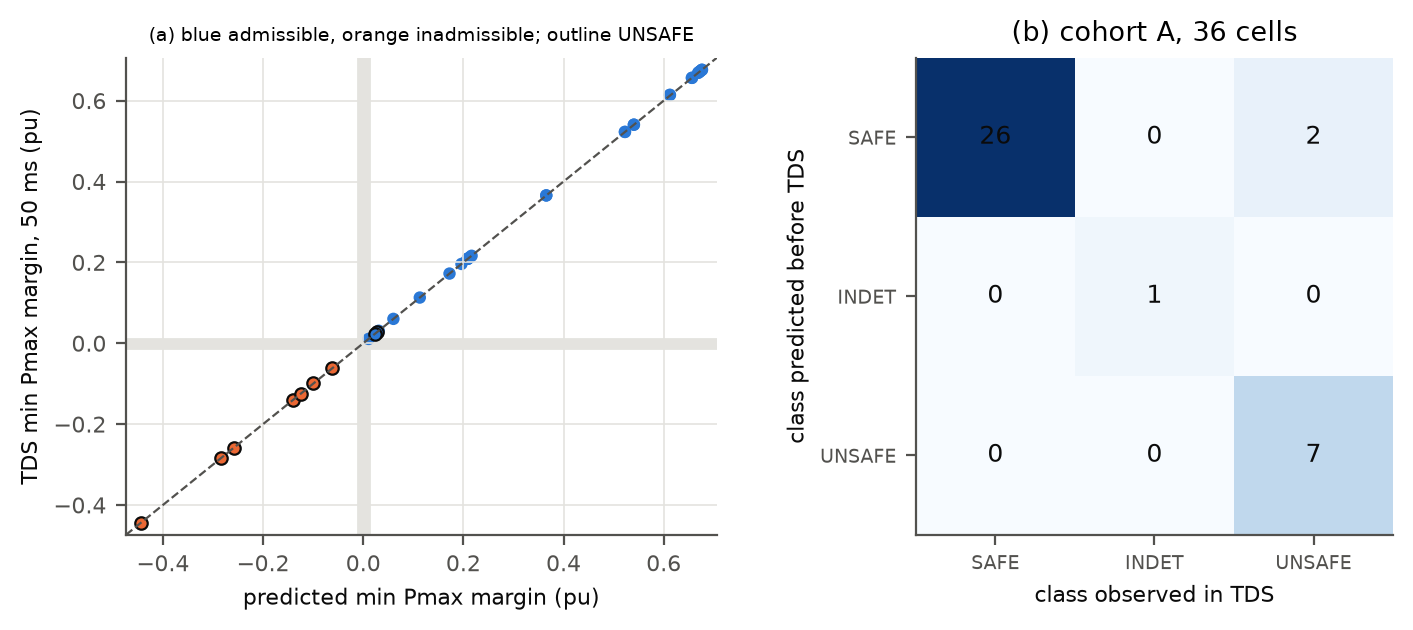
\includegraphics[width=\columnwidth]{figures_main/IEEE39_DEC062_F11_TEST_prediction_vs_TDS.png}
\caption{Predicted vs. observed margins and class table for the 36 blind cells.}
\label{fig:pred}
\end{figure}

\subsection{Criteria and pre-registered hypotheses}
Criterion (i) (no eligible UNSAFE cell) fails at OC1 (M0: five eligible cells, three inadmissible; rev3: b31 S2). Criterion (iv) passes in all eligible cells, narrowly for OC1 rev3 S3 (0.951 and 0.899~mpu). Hypotheses falsified: classes equal to predictions (34 of 36), $e\ge0$, and ``OC1 S3 cells fail (iv)'' (falsified in the favourable direction). Held: reference invariance without fallback, target verification, inadmissible cells never SAFE, null OC2 dispatch effect, and controller independence of the 50~ms margin (max difference $5.8\times10^{-5}$~pu in the minimum-Pmax margin).

\subsection{Reference invariance and stability checks}
In 42 of 42 runs of B5$'$ and B4$'$ the reference margins stay non-negative (minimum $0.024$~pu) without QP fallback, and the 42 targets satisfy the conditions of Theorem~\ref{thm:t2}; the Lyapunov value ends at most at $4.2\times10^{-4}$ of its first value in the 36 B5$'$ runs. B2 and B1s also never leave $\mathcal W$ (minimum margin $\ge0.147$~pu), so these observations do not discriminate the filter. In all 36 B5$'$ runs the loop is on the QP fast path (with $v=v_{\rm nom}$) after the last solver call, at most 4.29~s after the event.

\subsection{Controller comparison}
In six S2 cells with the same event, dispatch and solver (Table~\ref{tab:cmp}, Fig.~\ref{fig:cmp}), the centered controllers show a frequency nadir 4--6~mHz higher than B2 and B1s, B2 leaves a unit-voltage offset of 36--37~mpu and a frequency error of $2.4\times10^{-4}$~Hz at 200~s, and B1s has the lowest control effort and voltage offset. B5$'$ and B4$'$ are nearly identical. \emph{There is no dominant controller}, and the centered controllers use the supervisory target of A-INFO.
\begin{table*}[t]
\centering\small
\caption{Six S2 cells (OC1 rev3 and OC2 M3+OS, buses 21, 31, 39). Ranges over the cells.}
\label{tab:cmp}
\begin{tabular}{lcccc}
\toprule
Metric & B5$'$ & B4$'$ & B2 & B1s\\\midrule
Nadir (Hz) & 59.9759--59.9783 & $\approx$B5$'$ & 59.9717--59.9725 & 59.9725--59.9730\\
Frequency error at 200~s (Hz) & $\le4\times10^{-7}$ & $\approx$B5$'$ & $2.4\times10^{-4}$ & $\le10^{-7}$\\
Unit-voltage offset at 200~s (mpu) & 0.13--0.62 & $\approx$B5$'$ & 36.5--37.3 & 0.05--0.13\\
$P$ total variation (pu) & 1.64--1.76 & $\approx$B5$'$ & 2.14--2.74 & 0.60\\\bottomrule
\end{tabular}
\end{table*}
\begin{figure}[t]
\centering
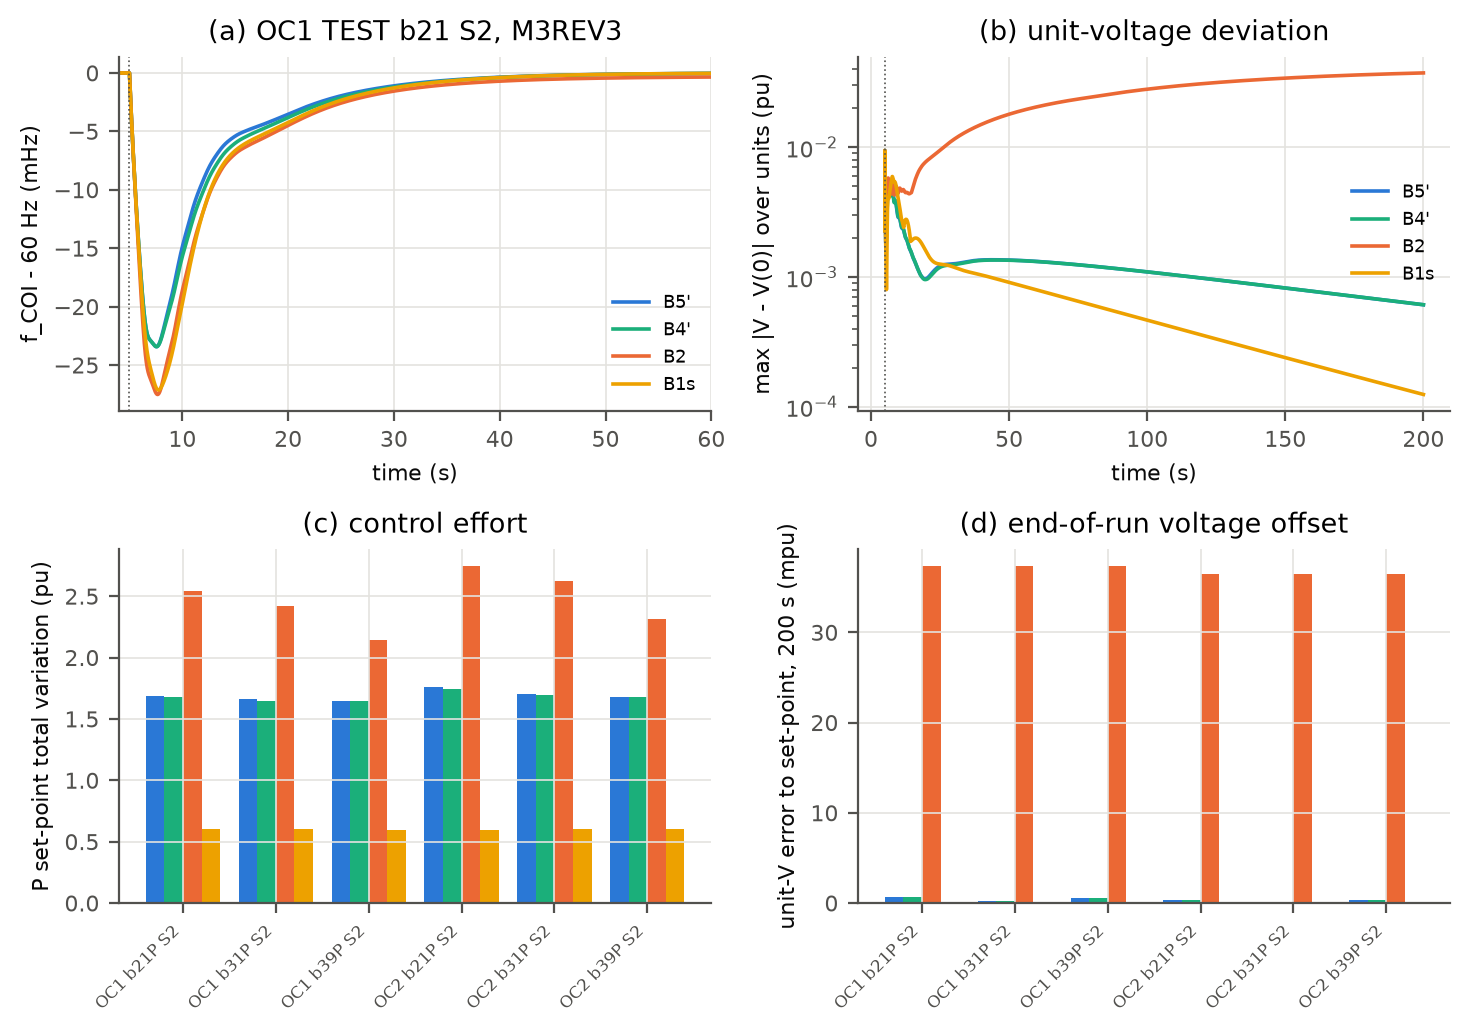
\includegraphics[width=\columnwidth]{figures_main/IEEE39_DEC062_F9_TEST_controller_comparison.png}
\caption{Controller comparison for OC1 rev3, bus 21, S2.}
\label{fig:cmp}
\end{figure}

\emph{Attribution.} Within the first second after the event, before the supervisory target is used, the total active-power reference moves $0.166$ (OC1) and $0.228$~pu (OC2) for B5$'$ and B4$'$ against $0.025$ for B2 and $0.027$ for B1s; in that interval the barrier rows cannot bind and the Lyapunov row is dropped, so by elimination the early difference arises from centering, not from the QP. The effect of the supervisory information on the later behaviour and on the 200~s offsets is not isolated experimentally. The dispatch effect is the only one measured with a single-factor contrast.

\subsection{Activity of the quadratic program}
The solver acts only in the first 4.3~s after the event; in 99.999\% of its calls the rate box is saturated; the box barrier rows cannot bind in the 33 runs at the rev3, OC2 M3+OS and OC2 M0 conditions (distance to binding $\ge0.113$~pu), and only in the nine OC1 M0 runs could the SG31 Pmax row bind (not observed; multipliers are not logged). The soft Lyapunov row is positive-slack in 32 of 36 runs. The difference between B5$'$ and B4$'$ is at most $14.1$~mpu in the active-power reference, $1.31$~mHz in frequency and $0.20$~mpu in unit voltage, and nil at 200~s (Fig.~\ref{fig:qp}). \emph{No benefit of the Lyapunov row is demonstrated.}
\begin{figure}[t]
\centering
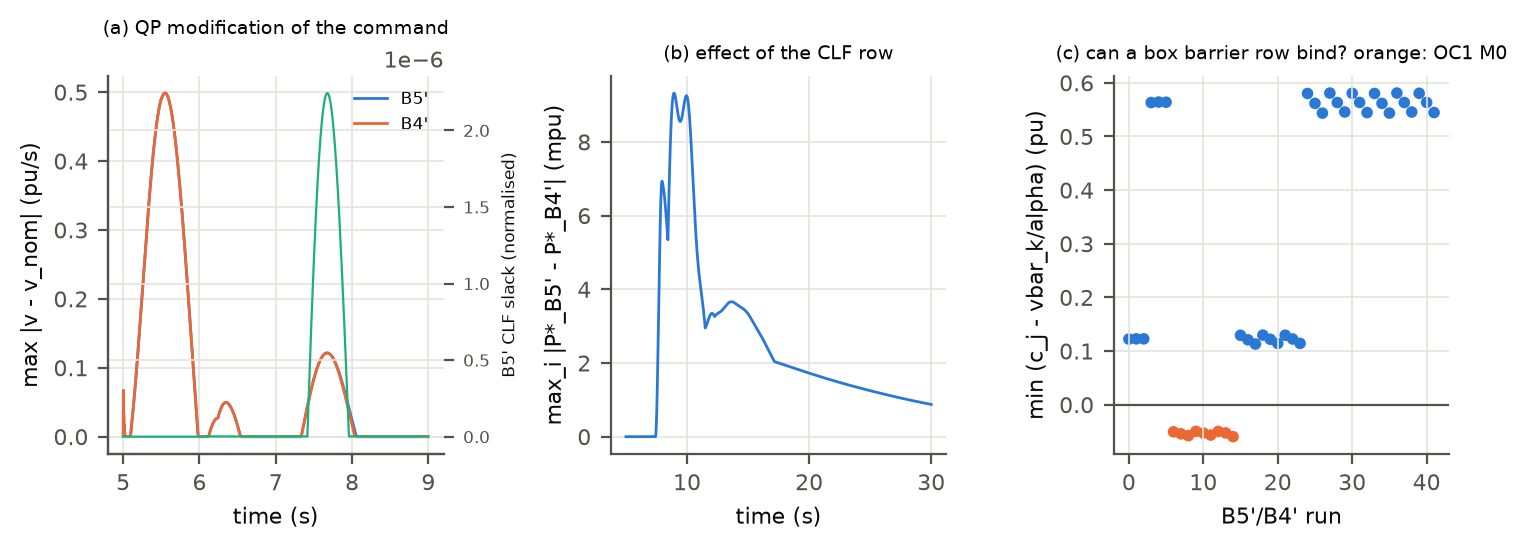
\includegraphics[width=\columnwidth]{figures_main/IEEE39_DEC063_F12_QP_activity.png}
\caption{QP activity and the difference between B5$'$ and B4$'$.}
\label{fig:qp}
\end{figure}

\subsection{Numerical check of the post-jump bound}
Section~\ref{sec:ta}, Remark~1(iii).

\subsection{Negative and limiting results}
The high-order barrier formulation of the original methodology is inapplicable in this plant (relative degree 3--4, no authority over two units, post-jump state outside the safe set); OC3 has an unstable target and is outside the hypotheses; bus 31 in OC1 is inadmissible for every controller of the class; G-v2 is rejected; three pre-registered hypotheses were falsified.

\section{Discussion, Limitations and Conclusions}
\label{sec:limits}
\textbf{What is established.} T-A and N2 are proved; Proposition~\ref{prop:os} is proved for the linearised plant and numerically validated; the dispatch effect on OC1 is observed in a single-factor contrast over three cells; Lemma~\ref{lem:c}, Theorem~\ref{thm:t1} and Theorem~\ref{thm:t2} are proved under the stated hypotheses.

\textbf{What is not claimed.} Universal or regional safety; regional or global stability; optimality of the dispatch or of the controller; a nonlinear bound for the influence of the controller after the jump; invariance of delivered quantities; protection of every bus; superiority of the proposed controller; any benefit of the quadratic program or of its Lyapunov row; novelty of reference invariance.

\textbf{Limitations.} A single network and plant model, step disturbances at three buses, two operating conditions with evidence on the dispatch in one of them; deterministic simulations (no variance); an access rule modified after tuning; a design revised after tuning; model-exact supervisory information; floating-point verification of the stability hypotheses; a literature search that is reproducible but not exhaustive (Sec.~\ref{sec:lit}).

\textbf{Conclusion.} The pre-event dispatch determines which events are admissible for any controller that respects continuity at the event; designing the dispatch for that instant improved the outcome in the cells where the event was admissible, and failed where it was not. The centered controller restores the selected equilibrium given the supervisory target, and the added optimisation layer did not show a measurable benefit.

\section*{Literature search note}
\label{sec:lit}
\todo{Replace by a short protocol statement: Crossref and arXiv queries of IEEE39\_DEC065\_search\_log.json (dates, filters), inclusion rules, works read in full, access limits (no IEEE Xplore, Scopus or Web of Science).}

\bibliographystyle{plain}
\bibliography{references,references_dec065}
\end{document}
